\documentclass[sigconf,nonacm]{acmart}
\usepackage{amsmath}
\usepackage{tikz}
\usetikzlibrary{positioning,arrows.meta,calc}
\settopmatter{printacmref=false}
\title{Generative Models as Recommendation Engines: A Survey of Architectures, Representations, and Learning Paradigms}
\author{Mingyu Lin}
\affiliation{%
  \institution{Shanghai Jiao Tong University}
  \city{Shanghai}
  \country{China}
}
\email{linmingyu@sjtu.edu.cn}   
\author{Shunyang Huang}                     
\affiliation{%
  \institution{Shanghai Jiao Tong University}
  \city{Shanghai}
  \country{China}
}
\email{syhuang123@sjtu.edu.cn}    
\settopmatter{printfolios=true}     
\begin{document}
\begin{abstract}
Generative recommendation has emerged as a promising approach that uses generative models to predict user preferences and generate recommendations. These models offer new ways to represent items and model user behavior beyond conventional candidate scoring and ranking. However, existing methods differ considerably in their objectives, output representations, and inference strategies, complicating comparisons of their relationships and practical trade-offs. In this survey, we review three major research directions: language-model-based recommendation, recommendation-specific generative systems, and diffusion-based recommendation. We compare representative methods in terms of item representation, learning objectives, generation strategies, and computational efficiency. We also discuss challenges in valid item generation, dynamic catalog maintenance, inference cost, and reliable evaluation. Through this comparison, we examine each paradigm's strengths, limitations, and integration into practical recommender systems. Our analysis clarifies recent advances in model-level generative recommendation and identifies directions for future research.
\end{abstract}
\maketitle

\section{Introduction}

Recommender systems play an important role in helping users discover relevant items from large and continuously evolving catalogs. Traditional recommender systems typically rely on a multi-stage pipeline consisting of candidate retrieval, ranking, and filtering. For example, the YouTube recommender system separates candidate generation from ranking to efficiently handle large-scale recommendations~\cite{youtube}. Although this architecture has proven effective, independently optimized stages may introduce inconsistencies between retrieval and ranking objectives. In particular, potentially relevant items can be excluded during early stages and cannot be recovered by subsequent ranking. Generative recommendation offers an alternative approach by using generative models to learn user preferences and generate recommendations. Instead of relying solely on scoring candidate items, these methods can generate item identifiers, recommendation sequences, or preference representations that are subsequently mapped to items in the catalog. This shift introduces new opportunities for recommendation modeling while also raising challenges in representation learning, inference, and system efficiency.

Recent advances in generative modeling have led to an increasing number of recommendation approaches. Language-model-based methods formulate recommendation as a language generation task, allowing models to use semantic information and pretrained knowledge. Recommendation-specific generative systems explore item tokenization, generative retrieval, and large-scale sequential modeling to produce recommendation outputs. Diffusion-based approaches provide another perspective by learning user preferences or item representations through iterative denoising. Although these methods share the goal of improving recommendation through generative modeling, they differ considerably in their output representations, learning objectives, and inference procedures. Existing surveys provide broad overviews of generative recommendation~\cite{survey,survey2026} or focus specifically on language-model-based approaches~\cite{llmsurvey}. However, a focused comparison of how different generative paradigms generate recommendations and function within practical recommendation pipelines remains valuable.

In this survey, we focus on \emph{model-level generative recommendation}, where generative models play a central role in producing recommendation decisions. This scope excludes methods used solely for data augmentation, feature extraction, or explanation generation. We review three major research directions: language-model-based recommendation, recommendation-specific generative systems, and diffusion-based recommendation. Representative approaches include P5~\cite{p5}, TIGER~\cite{tiger}, HSTU~\cite{hstu}, OneRec~\cite{onerec}, DiffRec~\cite{diffrec}, and DreamRec~\cite{dreamrec}, together with related studies on item tokenization, catalog grounding, and generative learning. We compare these approaches in terms of item representation, learning objectives, generation strategies, and computational efficiency. We also examine challenges related to valid item generation, dynamic item catalogs, inference costs, and reliable evaluation. To account for differences in experimental settings, we focus on the underlying technical distinctions and trade-offs among these methods.

Figure~\ref{fig:survey_overview} summarizes the organization of this survey. The three major research directions are organized into the subtopics examined in Section~\ref{sec:architectures}, with representative methods shown for each subtopic. We then compare these approaches in Section~\ref{sec:comparison} and discuss open challenges in Section~\ref{sec:challenges}.

\begin{figure*}[!t]
\centering
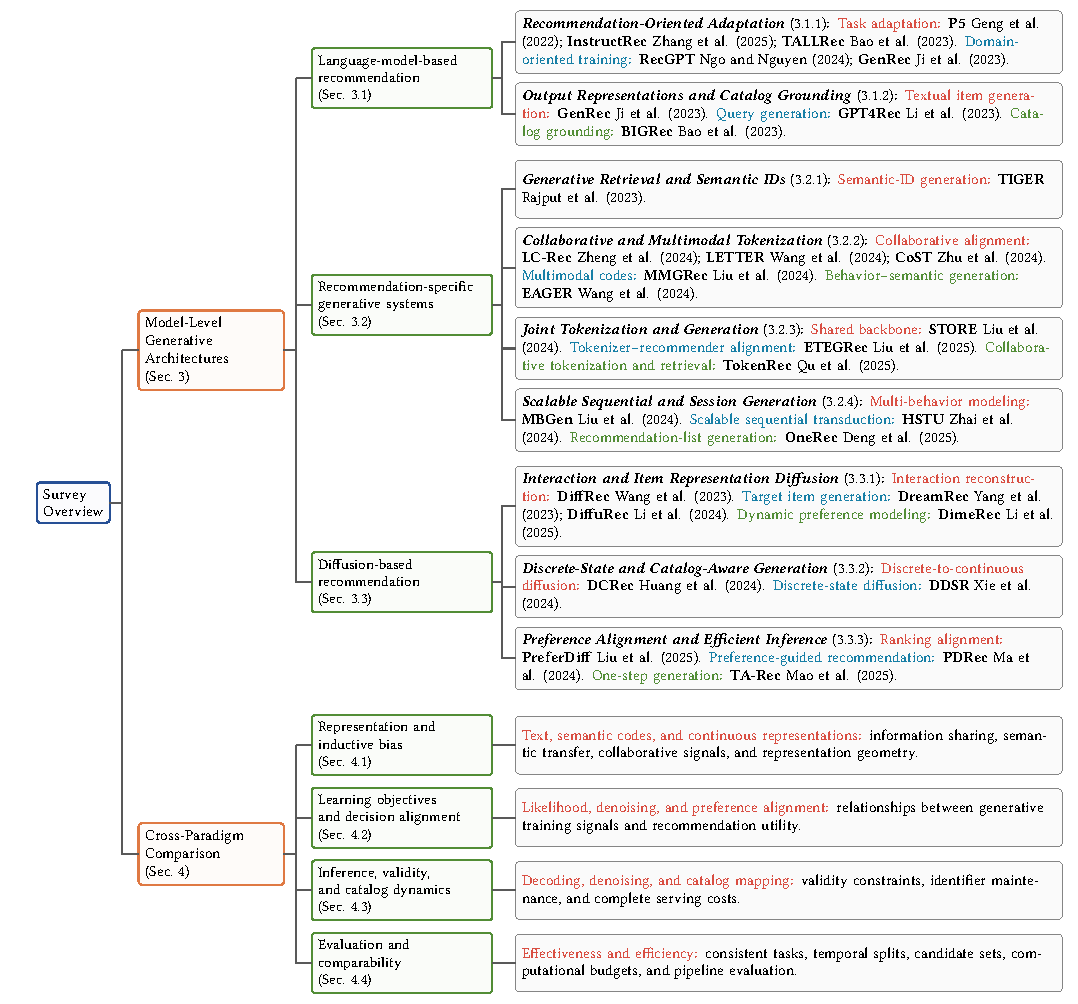
\includegraphics[width=\textwidth,height=.90\textheight,keepaspectratio]{figures/overview.pdf}
\caption{Taxonomy and organization of this survey. The tree follows the
sections on generative architectures and cross-paradigm comparison.
Representative methods are grouped by the architectural
subtopics reviewed in the text; colored labels identify their technical focus.
The grouping follows the survey structure, and related methods may span
multiple topics.}
\Description{A left-to-right tree rooted at Survey Overview. Two branches
represent generative architectures and cross-paradigm comparison.
The architecture branch expands into language-model-based,
recommendation-specific, and diffusion-based methods, with nine subtopic
boxes listing representative methods and author-year references. Four
comparison dimensions appear below.}
\label{fig:survey_overview}
\end{figure*}


\section{Background and Formulation}
\label{sec:background}

Let $\mathcal{I}$ denote the item catalog,
$h=(i_1,a_1,\ldots,i_t,a_t)$ a user's interaction history,
where $i_t$ and $a_t$ represent the interacted item and the
corresponding action, and $c$ the recommendation context.
Conventional recommendation methods typically learn a scoring
function $s_\theta(h,c,i)$ to estimate the relevance of a
candidate item $i\in\mathcal{I}$ to user preferences, and
produce recommendations through candidate retrieval and
ranking~\cite{youtube}.

Generative recommenders model user preferences using
$p_\theta(y\mid h,c)$, a conditional distribution over
recommendation-related outputs, where $y$ may represent a
natural-language item description, a discrete item identifier,
a sequence of semantic tokens, or a continuous preference
representation. For a discrete token sequence
$y=(y_1,\ldots,y_L)$, autoregressive models factorize the
conditional distribution as follows:
\begin{equation}
    p_\theta(y\mid h,c)
    =
    \prod_{j=1}^{L}
    p_\theta(y_j\mid y_{<j},h,c).
    \label{eq:autoregressive}
\end{equation}

Autoregressive approaches typically maximize the likelihood
of target sequences, whereas diffusion-based approaches learn
continuous user preference or item representations through
iterative denoising. Different generative mechanisms lead to
different recommendation procedures. Textual outputs and
discrete identifiers can be resolved to catalog items through
decoding and lookup, while continuous representations are
typically converted into recommendations through
similarity-based retrieval or preference-score ranking.
Figure~\ref{fig:paradigms} places these procedures side by
side: each paradigm produces a different intermediate output,
and a catalog-mapping step turns that output into the final
top-$K$ items.

\begin{figure*}[t]
\centering
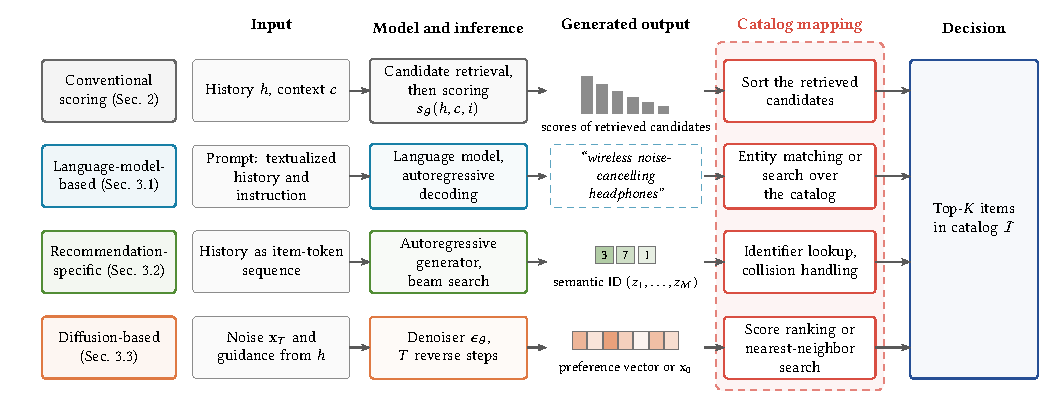
\includegraphics[width=\textwidth]{figures/paradigms.pdf}
\caption{Recommendation procedures of conventional scoring and
the three generative paradigms. The paradigms differ in what the
model generates and in how the generated output is mapped back to
items in the catalog (shaded column).}
\Description{Four rows, one per paradigm, each flowing from input
to model, generated output, catalog mapping, and a shared box of
top-K catalog items. Conventional scoring sorts candidate scores;
language models generate item text that is matched to the catalog;
recommendation-specific systems generate semantic IDs that are
looked up; diffusion models denoise a vector that is ranked or
matched by nearest-neighbor search.}
\label{fig:paradigms}
\end{figure*}

Generative modeling has a long history in recommender
systems. Mult-VAE~\cite{multvae} employs a
variational autoencoder to probabilistically model user
interactions and rank items using reconstructed preference
signals. SASRec~\cite{sasrec} and
BERT4Rec~\cite{bert4rec} learn sequential user
preferences through causal self-attention and bidirectional
contextual modeling, respectively, providing important
foundations for subsequent research on generative sequential
recommendation. With advances in language models, semantic
identifiers, and diffusion models, the generation targets of
recommender systems have expanded to item tokens,
recommendation sequences, and continuous latent
representations, giving rise to diverse generative modeling
paradigms.

This survey focuses on \emph{model-level generative
recommendation}, in which generative models directly
contribute to recommendation decisions. We examine three
major paradigms: language-model-based recommendation,
recommendation-specific generative systems, and
diffusion-based recommendation. The following sections
analyze these paradigms along four dimensions: output
representation, learning objective, inference mechanism,
and recommendation decision process, highlighting their
modeling characteristics and practical applicability.

\section{Model-Level Generative Architectures}
\label{sec:architectures}

This section reviews the three paradigms in turn.


\subsection{Language-Model-Based Recommendation}
\label{sec:lm}

Language-model-based recommendation formulates recommendation
tasks as conditional language generation, enabling user
interactions, item attributes, and task instructions to be
represented within a unified textual framework. This paradigm
leverages pretrained linguistic knowledge to capture semantic
relationships among items while learning personalized preferences
from interaction data. Existing approaches primarily differ in
how language models are adapted to recommendation tasks and
how generated outputs are mapped to actual catalog items.

\subsubsection{Recommendation-Oriented Adaptation}

P5~\cite{p5} establishes a unified text-to-text paradigm
that represents diverse recommendation tasks through personalized
prompts and trains a shared sequence-to-sequence model.
By expressing user interactions, item metadata, and prediction
targets in natural language, P5 enables different tasks to share
representations and learning objectives. This formulation
provides a flexible interface for recommendation, although
the quality of personalized predictions remains dependent on
the interaction signals available during training.

Subsequent research investigates how pretrained language models
can be adapted to recommendation-specific objectives.
InstructRec~\cite{instructrec} formulates recommendation as
instruction following, incorporating personalized requirements
into task descriptions to support diverse recommendation
scenarios. TALLRec~\cite{tallrec} adopts parameter-efficient
fine-tuning to align language models with recommendation
tasks using interaction data. These methods emphasize task
adaptation through instruction supervision, allowing general
language representations to support preference-oriented
prediction.

Another direction incorporates recommendation knowledge
more directly into model training. RecGPT~\cite{recgpt}
investigates domain-adapted generative pretraining
and instruction tuning, strengthening the connection between
language modeling and domain-specific data.
GenRec~\cite{genrec} fine-tunes a LLaMA-based model on
textualized user--item interactions and generates target items
from historical preferences. Unlike approaches that primarily
select among explicitly provided candidates, GenRec treats
item prediction as a language generation task.

These studies reveal two complementary strategies for
recommendation adaptation. Instruction-based methods emphasize
the correspondence between task descriptions and expected
outputs, whereas domain-oriented training incorporates
interaction patterns into the model's learned representations.
Their effectiveness depends on the integration of linguistic
semantics and collaborative preference signals. In particular,
semantic relationships derived from item descriptions provide
useful content information, while interaction histories capture
user-specific preferences that may not be fully expressed
through textual similarity.

\subsubsection{Output Representations and Catalog Grounding}

The output representation determines how language generation
is translated into recommendation decisions. Language-model-based
methods employ several forms of generated outputs, including
item titles, descriptive text, and search queries. These
representations provide different interfaces between the
language model and the underlying item catalog.

GenRec~\cite{genrec} uses textual item identities as generation
targets, allowing the model to associate recommendation outputs
with natural-language item information. GPT4Rec~\cite{gpt4rec}
adopts a different formulation by generating search queries
from user interaction histories and retrieving corresponding
items through a search engine. Its multi-query generation
strategy represents different aspects of user interests,
connecting generative preference modeling with conventional
information retrieval. The quality of the resulting
recommendations therefore reflects both the generated queries
and the retrieval mechanism.

BIGRec~\cite{bigrec} explicitly separates recommendation
generation from catalog grounding. It first adapts a language
model to generate recommendation-oriented item descriptions
and subsequently identifies corresponding catalog items.
This two-stage formulation connects the semantic flexibility
of language generation with the requirement that recommended
items belong to an existing catalog. It also highlights the
importance of the mapping mechanism in determining final
recommendation quality.

Different output interfaces introduce distinct representation
and inference characteristics. Natural-language descriptions
can exploit semantic knowledge acquired during pretraining,
but their correspondence to catalog entries may be ambiguous.
Item titles may be shared by multiple products, while
tokenization can produce variable-length representations.
Catalog grounding resolves generated text into identifiable
items through matching, retrieval, or ranking, introducing
additional decisions into the recommendation pipeline.
Consequently, the effectiveness of language-based recommendation
depends on both the quality of preference generation and the
accuracy of the grounding procedure.

Output representation also influences the scope of evaluation.
Candidate-based recommendation measures selection within a
specified item set, whereas full-catalog generation requires
the model and its grounding mechanism to identify relevant
items from the entire available catalog. Evaluating these
settings separately helps distinguish task adaptation from
retrieval capability. Existing benchmarks~\cite{llmbench}
further motivate assessing direct item selection alongside
other language-oriented recommendation tasks.

Overall, language-model-based recommendation offers a flexible
framework for combining semantic knowledge, personalized
interaction histories, and task-specific instructions.
Its central design choices concern the adaptation of linguistic
representations to collaborative preferences and the connection
between generated language and catalog-level decisions.
These considerations also motivate recommendation-specific
generative systems that replace natural-language outputs
with structured item representations, as discussed in the
following section.


\subsection{Recommendation-Specific Generative Systems}
\label{sec:rec}

Recommendation-specific generative systems represent items and
user interactions using structured tokens or learned
representations tailored to recommendation tasks. Unlike
language-oriented approaches that primarily rely on textual
outputs, these systems directly model item identities,
interaction sequences, or recommendation lists within
specialized output spaces. Their development has centered
on four closely related directions: semantic item
tokenization, collaborative representation learning,
joint optimization of tokenization and generation, and
scalable sequential generation.

\subsubsection{Generative Retrieval and Semantic IDs}

Generative retrieval reformulates candidate retrieval as
the prediction of item identifiers conditioned on user
interaction histories. TIGER~\cite{tiger} establishes
this paradigm by representing each item as a sequence
of discrete semantic tokens derived from its content
embedding. A sequence-to-sequence Transformer then
generates the semantic identifier of a relevant item
autoregressively, replacing independent candidate
scoring with token-level prediction.

The construction of semantic identifiers typically
relies on residual vector quantization. Given an item
embedding $\mathbf{e}_i$, a sequence of codebook
vectors is selected to approximate its representation:
\begin{equation}
    \mathbf{e}_i \approx
    \sum_{m=1}^{M}
    \mathbf{c}_{m,z_{i,m}},
    \label{eq:semantic_quantization}
\end{equation}
where $M$ denotes the number of quantization levels,
$z_{i,m}$ is the code index assigned to item $i$ at
level $m$, and $\mathbf{c}_{m,z_{i,m}}$ is its
corresponding codebook vector. Each level quantizes
the residual left by preceding levels. RQ-VAE~\cite{rqvae}
learns such hierarchical representations through
reconstruction and quantization objectives.

The resulting identifier
$(z_{i,1},\ldots,z_{i,M})$ provides a compact
representation of item identity. Items with related
representations may share code prefixes, enabling
statistical sharing across items during autoregressive
prediction. At inference, beam search generates
candidate code sequences, which are resolved into
catalog items through identifier lookup. Additional
disambiguation is used when multiple items receive
the same semantic codes. Figure~\ref{fig:semantic_id}
illustrates both steps.

\begin{figure}[t]
\centering
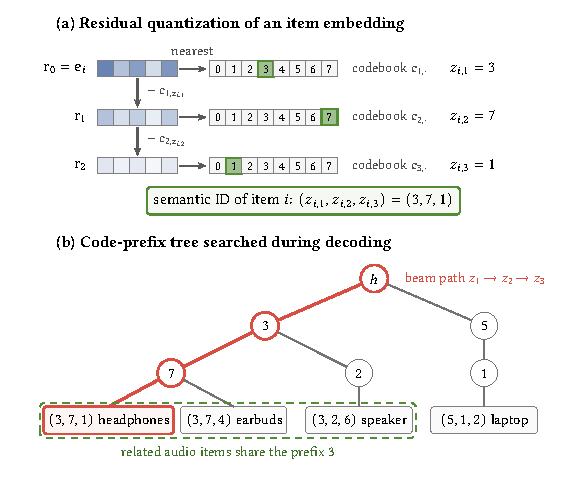
\includegraphics[width=\columnwidth]{figures/semantic_id.pdf}
\caption{Semantic identifiers. (a) Each level selects the
nearest codebook vector and passes the residual to the next
level. (b) Related items share code prefixes, and decoding
follows a beam path through the prefix tree to a valid item.}
\Description{Top: an item embedding is quantized over three
levels, giving the code (3, 7, 1). Bottom: a prefix tree from the
user history through codes to four items; headphones, earbuds, and
a speaker share prefix 3, and the highlighted beam path reaches
headphones.}
\label{fig:semantic_id}
\end{figure}

This formulation connects representation learning
with generative retrieval: the tokenizer determines
the structure of the prediction space, while the
generator learns the conditional distribution over
item codes. Consequently, retrieval effectiveness
depends on both the semantic structure of the
identifiers and the probability assigned to their
token sequences. Codebook capacity, identifier
collisions, and decoding strategies jointly affect
retrieval accuracy and computational efficiency.

\subsubsection{Collaborative and Multimodal Tokenization}

Early semantic tokenization primarily emphasizes
content-derived item representations. Subsequent
research incorporates collaborative signals to
better align item identifiers with personalized
recommendation objectives.

LC-Rec~\cite{lcrec} addresses the gap between
linguistic semantics and collaborative preferences
by learning discrete item indices through vector
quantization and introducing alignment tasks that
connect item codes, language representations, and
user interactions. The resulting identifiers provide
a structured interface through which language models
can incorporate collaborative information into
item generation.

LETTER~\cite{letter} further investigates the
representation properties required for effective
generative recommendation. Its tokenization framework
combines hierarchical semantic regularization,
collaborative alignment, and code-assignment diversity.
The semantic objective preserves relationships among
item representations, collaborative supervision
incorporates interaction patterns, and diversity
regularization encourages more balanced code usage.
LETTER also introduces a ranking-guided generation
objective to connect token prediction with
recommendation relevance.

Related approaches explore alternative mechanisms
for integrating collaborative structure.
CoST~\cite{cost} incorporates contrastive item
relationships into the quantization process,
providing additional supervision beyond embedding
reconstruction. MMGRec~\cite{mmgrec} constructs
item identifiers through graph-aware residual
quantization of multimodal and collaborative
representations, and subsequently generates these
identifiers autoregressively. These methods extend
semantic tokenization beyond content similarity
toward preference-aware item representations.

The integration of heterogeneous information can
also occur at the generation stage. EAGER~\cite{eager}
employs a shared encoder with separate behavioral
and semantic decoders. The two streams generate
complementary item representations, which are
combined through confidence-based ranking. Whereas
LETTER, CoST, and MMGRec emphasize the construction
of informative item codes, EAGER incorporates
behavioral and semantic information through
parallel generative pathways.

Item indexing itself introduces another design
dimension. Comparative experiments using the P5
backbone~\cite{indexids} demonstrate that different
identifier schemes, including random, sequential,
collaborative, and semantic representations, can
substantially influence recommendation performance.
IDGenRec~\cite{idgenrec} explores concise textual
identifiers that preserve linguistic meaning while
representing item identity. These indexing strategies
connect identifier structure with the information
available to the generative model.

Taken together, these studies establish item
tokenization as an important component of
generative recommendation whose effects extend
beyond preprocessing. Effective identifiers
must balance semantic information, collaborative
relevance, code distinguishability, and generation
efficiency. Empirical analyses such as
GRID~\cite{grid} further highlight the importance
of implementation choices and component-level
evaluation in semantic-ID-based recommendation.

\subsubsection{Joint Tokenization and Generation}

Conventional semantic-ID pipelines often optimize
item tokenization and recommendation generation
in separate stages. The tokenizer learns a discrete
representation from item features, after which a
generative model is trained to predict the assigned
codes. This separation simplifies training but
introduces a potential mismatch between
representation fidelity and predictive utility:
codes that reconstruct item embeddings accurately
may not be optimal for prediction from user histories.

Recent approaches address this mismatch through
closer integration of representation learning and
recommendation objectives. STORE~\cite{store}
formulates semantic tokenization and generative
recommendation within a shared language-model
backbone. It unifies text-to-token and token-to-token
generation with auxiliary reconstruction tasks,
allowing item representation learning and
recommendation prediction to share model parameters.

ETEGRec~\cite{etegrec} couples an item tokenizer
with a generative recommender through two
complementary alignment objectives.
Se\-quence--\allowbreak item alignment connects generated
sequence representations with target items, while
preference--\allowbreak semantic alignment relates collaborative
preferences to item semantics. Alternating optimization
coordinates the two components, enabling token
representations to evolve with the recommendation
objective.

TokenRec~\cite{tokenrec} approaches the problem
through collaborative tokenization and efficient
retrieval. It quantizes masked user and item
representations learned from collaborative information,
while introducing a retrieval mechanism that avoids
conventional autoregressive beam decoding.
Its design connects the quality of discrete
representations with the computational requirements
of top-$K$ recommendation.

These methods represent complementary directions
for improving the relationship between tokenization
and generation. STORE emphasizes architectural
sharing, ETEGRec optimizes the interaction between
separate components, and TokenRec jointly considers
collaborative token construction and retrieval
efficiency. Their differences indicate that
representation quality should be assessed through
downstream recommendation performance and decoding
cost, in addition to embedding reconstruction.

Another consideration is the stability of item
identifiers as catalogs evolve. Updating learned
codebooks may change the token sequences associated
with existing items, affecting previously learned
generation patterns. Maintaining stable identifiers,
incorporating newly introduced items, and updating
catalog mappings therefore form part of the
representation-learning problem. These requirements
connect tokenizer design with the long-term
operation of generative recommendation systems.

\subsubsection{Scalable Sequential and Session Generation}

Beyond item representation, recent generative
systems investigate how recommendation objectives
and model architectures can support heterogeneous
behaviors, long interaction histories, and
list-level prediction.

MBGen~\cite{mbgen} extends autoregressive
recommendation to multi-behavior interaction
sequences. It interleaves behavior and item tokens
and models recommendation as a two-stage prediction
process: generating the next behavior type and
subsequently predicting an item conditioned on
that behavior. A position-routed sparse architecture
supports efficient modeling of the heterogeneous
token sequence. This formulation incorporates
behavioral intent directly into the generative
prediction objective.

HSTU~\cite{hstu} investigates the scalability
of sequential recommendation through a
generative transduction framework. Its hierarchical
sequential transduction units are designed for
high-cardinality, nonstationary interaction data,
with architectural and serving optimizations
supporting long histories and large-scale
computation. Unlike semantic-ID retrieval models,
HSTU primarily advances the modeling and
computational efficiency of user action sequences.
It illustrates how generative sequential modeling
can be integrated into industrial recommendation
architectures without requiring the same
identifier-generation interface as TIGER.

OneRec~\cite{onerec} extends generative
recommendation from candidate retrieval toward
unified recommendation-list generation. Its
encoder--decoder architecture generates sequences
of recommended items, while a sparse
mixture-of-experts design increases model capacity.
The system further introduces iterative preference
alignment to optimize generated sessions according
to learned preference signals.

The distinction between next-item and session-level
generation can be expressed through the probability
of an ordered recommendation list
$Y=(i_1,\ldots,i_K)$:
\begin{equation}
    p_\theta(Y\mid h)
    =
    \prod_{k=1}^{K}
    p_\theta(i_k\mid h,i_{<k}).
    \label{eq:session_generation}
\end{equation}
Here, each generated item is conditioned on the
interaction history and preceding recommendations.
This factorization allows list generation to model
dependencies among recommended items, including
complementarity, substitution, and redundancy.
It therefore extends the prediction target
from individual item relevance to the structure
of an entire recommendation sequence.

OneRec~\cite{onerec} further incorporates
iterative preference alignment based on direct
preference optimization~\cite{dpo}. A reward model
evaluates generated sessions and provides
preference comparisons for optimizing the
relative likelihood of preferred and rejected
sequences. This mechanism supplements
sequence-likelihood training with feedback
associated with session-level recommendation
quality.

Scalability and integration take several forms
in these systems. MBGen expands
the behavioral information represented in
generative sequences, HSTU addresses the
computational demands of large-scale interaction
modeling, and OneRec extends generation toward
list-level recommendation and preference alignment.
Together, they demonstrate the progression
from item-oriented generative retrieval toward
more expressive recommendation objectives
and integrated serving architectures.

Overall, recommendation-specific generative
systems advance the field along two complementary
axes: learning structured representations that
support accurate item generation, and developing
generative architectures that capture increasingly
complex recommendation decisions. Their practical
effectiveness depends on the interaction among
identifier design, learning objectives, decoding
strategies, and system-level efficiency.


\subsection{Diffusion-Based Recommendation}
\label{sec:diffusion}

Diffusion-based recommendation models user preferences and
item representations through a progressive denoising process.
Unlike autoregressive approaches that generate discrete
tokens sequentially, diffusion models learn to recover
recommendation-related signals from corrupted observations.
For a continuous target $\mathbf{x}_0$, a standard Gaussian
forward process~\cite{ddpm} is defined as
\begin{equation}
    q(\mathbf{x}_t \mid \mathbf{x}_0)
    =
    \mathcal{N}\left(
    \sqrt{\bar{\alpha}_t}\mathbf{x}_0,
    (1-\bar{\alpha}_t)\mathbf{I}
    \right),
    \label{eq:diffusion_forward}
\end{equation}
where $\bar{\alpha}_t$ denotes the cumulative noise
schedule. A parameterized denoising model learns to
reverse this corruption process, optionally conditioned
on user interaction histories. Depending on the target
representation, the resulting outputs can be reconstructed
interaction scores, item embeddings, or preference
representations used to derive recommendations.

\subsubsection{Interaction and Item Representation Diffusion}

Early diffusion-based recommenders explore generative
modeling of user--item interactions. DiffRec~\cite{diffrec}
applies diffusion to interaction vectors and reconstructs
personalized preference signals for item ranking.
Its forward process introduces controlled noise to
preserve informative interaction patterns during
denoising. To address the characteristics of
recommendation data, DiffRec further introduces
two extensions. L-DiffRec compresses item dimensions
through clustering and latent-space diffusion,
while T-DiffRec incorporates temporal information
through interaction reweighting. These designs
adapt diffusion to large item spaces and evolving
user preferences.

Another research direction generates representations
of target items conditioned on historical interactions.
DreamRec~\cite{dreamrec} reformulates sequential
recommendation as conditional item generation.
A Transformer encodes the user's interaction history
into a guidance representation, which conditions the
reverse diffusion process to generate an embedding
corresponding to a preferred next item. The generated
representation is subsequently matched with catalog
items through embedding similarity. This formulation
shifts the prediction target from candidate relevance
scores to a distribution over desirable item
representations.

DiffuRec~\cite{diffurec} similarly employs diffusion
for sequential recommendation, but emphasizes
uncertainty in item representations. It models
target items through distributions that capture
multiple item aspects and user interests.
Historical interactions guide the reconstruction
of target item representations, followed by a
rounding operation that identifies discrete items.
Together, DreamRec and DiffuRec demonstrate how
conditional diffusion can represent personalized
preferences beyond fixed item embeddings.

DimeRec~\cite{dime} further investigates the
interaction between generative modeling and
nonstationary user interests. It combines a
guidance extraction module with a diffusion-based
aggregation module. The former extracts stable
guidance signals from evolving interaction
histories, while the latter generates preference
representations conditioned on these signals.
This design integrates multi-interest modeling
with diffusion-based representation generation.

These approaches differ primarily in their
generation targets and conditioning mechanisms.
DiffRec reconstructs interaction-level preferences,
whereas DreamRec and DiffuRec generate
representations associated with target items.
DimeRec emphasizes the aggregation of dynamic
user interests. The choice of target space
determines how denoised outputs are converted
into item rankings or recommendations.

\subsubsection{Discrete-State and Catalog-Aware Generation}

Continuous diffusion models operate in learned
representation spaces, while recommendation
decisions ultimately concern discrete catalog
items. Recent methods investigate this connection
through explicit item mapping and discrete-state
diffusion.

DCRec~\cite{dcrec} introduces a discrete-to-continuous
diffusion framework for sequential recommendation.
It extends the generative process to model the
transition between continuous item representations
and discrete item indices. Its dual conditional
diffusion Transformer incorporates implicit and
explicit conditioning to capture historical
preferences. This formulation integrates
item-level prediction more closely with the
diffusion process.

DDSR~\cite{ddsr} explores an alternative approach
by modeling diffusion directly in a discrete
state space. Motivated by uncertainty in
sequential user behavior, DDSR represents
interaction sequences through fuzzy sets and
employs discrete transition processes to
model evolving interests. To manage the large
state space associated with item identities,
it introduces compact semantic labels obtained
through quantization.

These methods extend diffusion-based recommendation
beyond conventional continuous embedding
generation. DCRec connects continuous denoising
with discrete item prediction, whereas DDSR
models transitions over discrete semantic states.
Their designs highlight the importance of
representation granularity and state-space
construction in connecting generative processes
with catalog-level recommendation decisions.

\subsubsection{Preference Alignment and Efficient Inference}

A central challenge in diffusion-based recommendation
is the relationship between denoising objectives
and personalized ranking quality. A common
noise-prediction objective minimizes
\begin{equation}
    \mathcal{L}_{\mathrm{denoise}}
    =
    \mathbb{E}_{t,\mathbf{x}_0,\boldsymbol{\epsilon}}
    \left[
    \left\|
    \boldsymbol{\epsilon}
    -
    \boldsymbol{\epsilon}_{\theta}
    (\mathbf{x}_t,t,h)
    \right\|_2^2
    \right],
    \label{eq:diffusion_denoise}
\end{equation}
where $\boldsymbol{\epsilon}$ denotes sampled
Gaussian noise and $h$ represents the
interaction history. Although denoising
objectives support distribution learning,
reconstruction accuracy and recommendation
relevance capture different aspects of
model performance.

PreferDiff~\cite{preferdiff} addresses this
relationship by incorporating personalized
ranking into diffusion learning. It reformulates
Bayesian personalized ranking within a
generative likelihood framework and introduces
multiple negative samples to capture relative
item preferences. Variational optimization
and cosine-based error further connect
diffusion learning with ranking objectives.
This approach integrates preference-aware
supervision into the generative training
process.

Diffusion-generated preferences can also
support existing sequential recommenders.
PDRec~\cite{pdrec} employs a diffusion model
as a plug-in component to estimate dynamic
user preferences. It uses these signals
for historical behavior reweighting,
positive-sample augmentation, and
negative-sample selection. This design
uses diffusion-based preference modeling to
enhance downstream recommendation
without directly generating the final item.

Inference efficiency constitutes another
important research direction. Conventional
diffusion sampling often involves multiple
denoising steps, creating computational
overhead in latency-sensitive recommendation
settings. TA-Rec~\cite{tarec} addresses this
trade-off through a two-stage framework
for one-step generation. Temporal consistency
regularization is employed during pretraining
to encourage consistency across denoising
steps, while adaptive preference alignment
during fine-tuning improves the correspondence
between generated representations and user
preferences.

These methods address complementary aspects
of diffusion-based recommendation.
PreferDiff focuses on aligning generative
learning with ranking objectives, PDRec
integrates generated preference signals
into sequential recommendation, and TA-Rec
improves the efficiency of the generation
process. Their contributions connect
diffusion modeling with recommendation
utility and practical inference requirements.

Overall, diffusion-based recommendation
provides a distributional modeling
framework for generating interaction
preferences, target item representations,
and discrete recommendation states.
The development of this paradigm has
progressed from preference reconstruction
toward conditional generation, structured
item modeling, and preference-aware
optimization. Its effectiveness depends
on the interaction among generation
targets, conditioning information,
learning objectives, and inference
efficiency.


\section{Cross-Paradigm Comparison}
\label{sec:comparison}

The three generative paradigms differ in their output
representations, learning objectives, and mechanisms for
producing catalog-level recommendations. These distinctions
influence both the statistical properties of the models
and their computational requirements. The following comparison
examines their generation targets, learning signals, inference
procedures, and principal trade-offs.


\subsection{Representation and Inductive Bias}

The representation of recommendation targets determines
the structure of the prediction space and the information
shared across items. Natural-language representations
leverage semantic knowledge acquired during pretraining,
allowing models to associate user preferences with item
descriptions and attributes. Their effectiveness depends
on the correspondence between textual expressions and
catalog identities, particularly when item names are
ambiguous or descriptions are incomplete.

Semantic identifiers provide a more structured
alternative. By representing items as sequences of
discrete codes, methods such as TIGER~\cite{tiger}
and LC-Rec~\cite{lcrec} replace large atomic item
vocabularies with compositional token representations.
Shared code prefixes enable parameter sharing across
related items, while the learned code structure
introduces inductive biases into the generative
prediction process. Collaborative and multimodal
tokenization further incorporate behavioral relationships
that may differ from content-based similarity.

Continuous representations offer another modeling
perspective. Diffusion-based approaches generate
interaction preferences or target item embeddings
within continuous spaces, where similarity is
determined by the learned representation geometry.
DiffRec~\cite{diffrec} reconstructs interaction-level
signals, whereas DreamRec~\cite{dreamrec} generates
embeddings associated with preferred items.
The quality of the resulting recommendations
depends on both the generated representation
and its correspondence to catalog items.

These representation choices establish different
forms of generalization. Text supports transfer
from linguistic knowledge, semantic codes
encourage information sharing through structured
identifiers, and continuous embeddings support
distributional modeling in latent spaces.
Their respective advantages depend on the
availability of semantic features, collaborative
signals, and the structure of user preferences.

\subsection{Learning Objectives and Decision Alignment}

The learning objectives of generative recommenders
reflect different assumptions about how user
preferences should be modeled. Autoregressive
approaches typically maximize the conditional
likelihood of target item sequences. For semantic-ID
generation, this objective decomposes item prediction
into successive token-level decisions, allowing
statistical dependencies to be learned across
identifier components.

Diffusion-based approaches instead optimize
reconstruction or denoising objectives. These
objectives encourage models to recover interaction
patterns or target representations from corrupted
observations. However, representation reconstruction
and recommendation ranking optimize different
quantities. In particular, small errors in an
embedding space may change the nearest catalog
item, while accurate reconstruction of historical
interactions may not directly improve future
recommendation relevance.

Preference-oriented training introduces additional
supervision to connect generative learning with
recommendation utility. PreferDiff~\cite{preferdiff}
incorporates pairwise preference modeling into
diffusion learning, while OneRec~\cite{onerec}
uses iterative preference alignment to optimize
generated recommendation sessions. These
approaches extend the training signal beyond
the likelihood or reconstruction of observed
behavior toward relative preference estimation.

A common consideration across these objectives
is the relationship between observed interactions
and underlying user preferences. Historical
feedback reflects both user interests and
the exposure policies under which items were
presented. Consequently, likelihood estimation,
denoising reconstruction, and preference alignment
capture different aspects of the recommendation
problem. Their effectiveness is ultimately
determined by the correspondence between
training objectives and the quality of the
resulting recommendation decisions.

\subsection{Inference, Validity, and Catalog Dynamics}

The output representation also determines the
operations required during inference. Language-based
methods generate textual descriptions or queries
that must be resolved through matching or retrieval.
Semantic-ID models generate structured token
sequences and use identifier lookup to recover
catalog items. Diffusion models typically require
denoising followed by preference-score ranking
or similarity-based retrieval, while discrete-state
diffusion employs transitions over learned
semantic states.

These inference procedures introduce distinct
computational characteristics. Autoregressive
decoding cost depends on sequence length and search
strategy, with beam search increasing candidate
exploration at additional computational cost.
Diffusion inference depends on the number of
denoising steps and the complexity of the generated
representation. Models such as TA-Rec~\cite{tarec}
reduce this cost through one-step generation.
Sequential architectures such as HSTU~\cite{hstu}
instead emphasize efficient computation over
large-scale interaction histories.

The generated outputs must ultimately satisfy
catalog-level constraints. Textual outputs require
entity resolution, semantic codes require valid
identifier mappings, and continuous embeddings
require a decision rule for selecting discrete
items. Catalog filtering, deduplication, and
candidate ranking may therefore remain part of
the serving pipeline regardless of the
underlying generative paradigm.

Catalog evolution further connects representation
design with system maintenance. New items can
be incorporated into embedding indexes when
suitable representations are available, whereas
semantic-ID systems additionally require code
assignment and identifier management. Changes
to learned codebooks may affect previously
established item mappings. Text-based approaches
can exploit newly available descriptions, while
their retrieval quality depends on the
corresponding catalog index.

The practical efficiency of generative
recommendation should therefore be evaluated
at the system level. Relevant costs include
model execution, decoding or denoising,
catalog mapping, filtering, and any subsequent
ranking operations. This perspective provides
a common basis for comparing architectures
with substantially different inference procedures.

\subsection{Evaluation and Cross-Paradigm Comparability}

A meaningful comparison across generative
paradigms requires consistent recommendation
tasks and evaluation settings. Models may
produce the same number of final recommendations
while performing substantially different amounts
of intermediate computation. For example, a
semantic-ID generator may explore multiple
decoding paths, whereas a diffusion model may
generate a continuous representation and
retrieve its nearest catalog items. Comparing
their final top-$K$ results alone does not
capture these differences.

Evaluation should therefore distinguish
recommendation effectiveness from inference
efficiency. Ranking metrics such as Recall@$K$
and NDCG@$K$ measure the relevance of final
recommendation lists, while latency, throughput,
and memory consumption characterize serving
requirements. Reporting recommendation quality
under comparable computational budgets offers
further insight into the trade-offs among
generative paradigms.

The candidate universe and evaluation protocol
also influence reported performance. Candidate-based
prediction evaluates selection within a restricted
set, whereas full-catalog retrieval requires
identifying relevant items among all eligible
catalog entries. Comparisons should use consistent
temporal splits, interaction histories, catalog
snapshots, and candidate eligibility rules.
When sampled candidates are used for evaluation,
the sampling procedure and candidate-set size
should be reported explicitly.

Representation construction introduces further
considerations for temporal evaluation.
Semantic tokenizers and item embedding models
may use information that becomes available
at different stages of the recommendation
process. Separating training-period interactions
from future behavioral signals is necessary
to assess generalization under realistic
catalog conditions. Performance on new items
and long-tail items can additionally reveal
differences that aggregate ranking metrics
may obscure.

Finally, comparisons should account for the
complete recommendation pipeline, including
interactions among its components. Generative retrieval,
catalog grounding, reranking, and preference
alignment may be optimized separately or
jointly, leading to different degrees of
system integration. Evaluating final recommendation
quality alongside intermediate validity,
decoding cost, and serving efficiency provides
a more comprehensive characterization of
each approach.

Overall, the three paradigms make distinct
design choices and use generation mechanisms
that are not directly interchangeable. Language-based methods
emphasize semantic flexibility. Recom\-men\-dation-specific
generative systems exploit structured
item representations and sequential prediction.
Diffusion-based approaches model preferences
through denoising and distributional generation.
Their relative effectiveness depends on how
representation learning, optimization objectives,
inference mechanisms, and catalog decisions
are coordinated within the complete
recommendation system.


\section{Open Challenges and Research Directions}
\label{sec:challenges}

Despite recent advances, generative recommendation faces
several challenges in representation learning, preference
modeling, inference efficiency, and practical deployment.
We highlight six directions for future research.

\paragraph{Adaptive representations and catalog evolution.}
Dynamic catalogs require stable item representations while
accommodating newly introduced items. Semantic-ID methods
face code collisions, uneven code utilization, and
identifier changes. Future research should explore
incremental tokenization, stable codebooks, and the
integration of semantic and collaborative information
to improve cold-start and long-tail recommendation.

\paragraph{Valid and controllable generation.}
Generated outputs must correspond to available items
and satisfy user and application constraints.
Promising directions include catalog-aware decoding,
constraint-aware generation, and list-level optimization.
These mechanisms should jointly consider recommendation
relevance, validity, diversity, and catalog coverage.

\paragraph{Preference alignment and feedback modeling.}
Generative objectives based on interaction likelihood
or denoising reconstruction may differ from actual
recommendation utility. Future work could investigate
preference-aware learning, uncertainty-aware reward
modeling, and multi-objective optimization to better
align generated recommendations with user preferences
and long-term outcomes.

\paragraph{Efficient inference.}
Autoregressive decoding and iterative denoising introduce
computational overhead in large-scale recommendation.
Adaptive decoding, model distillation, and efficient
sampling offer promising directions for reducing latency.
Joint optimization of generation and catalog retrieval
may further improve end-to-end efficiency.

\paragraph{Reliable evaluation and reproducibility.}
Fair comparison requires consistent temporal splits,
candidate sets, and computational budgets.
Model-scaling studies~\cite{scaling} and analyses of
sampled ranking metrics~\cite{samplemetrics} highlight
important evaluation considerations. Future benchmarks
should incorporate cold-start performance, exposure bias,
generation validity, and computational efficiency.
Language-based methods additionally require evaluation
of history sensitivity and output reliability~\cite{beyondutility}.

\paragraph{Privacy and trustworthy deployment.}
Rich interaction histories introduce risks of sensitive
information exposure and model memorization.
Privacy-preserving learning, access control, and
reliable output filtering are important directions
for developing trustworthy generative recommenders.


\section{Conclusion}
\label{sec:conclusion}

This survey systematically reviewed three major paradigms
of generative recommendation: language-model-based approaches,
recommendation-specific generative systems, and diffusion-based methods.
Through a comparative analysis of their representations,
learning objectives, and inference mechanisms, we identified
the distinct modeling characteristics and practical trade-offs
of each paradigm. A central finding is that recommendation
effectiveness depends not only on generative modeling
capabilities but also on how generated outputs are mapped
to catalog items and aligned with user preferences.
Future research should emphasize adaptive representations,
preference-aware optimization, and efficient generation,
supported by rigorous evaluation under realistic
recommendation settings.


\balance
\bibliographystyle{ACM-Reference-Format}
\bibliography{references}
\end{document}
